\documentclass[11pt]{article}
\usepackage[margin=1in]{geometry}
\usepackage{amsmath, amssymb}
\usepackage{graphicx}
\usepackage{hyperref}
\usepackage{booktabs}
\usepackage{xcolor}
\usepackage{microtype}

\hypersetup{
    colorlinks=true,
    linkcolor=blue!60!black,
    citecolor=blue!60!black,
    urlcolor=blue!60!black,
}

\title{Local Importance-Gated Plasticity in Context-Modulated Physical Networks:\\
       \large Project Introduction and Current Baselines}
\author{Sonali Goel}
\date{May 2026}

\begin{document}
\maketitle

\begin{abstract}
This project studies continual learning in a physical-learning substrate:
a passive, edge-coupled resistor-like mesh trained by contrastive local
updates. The motivating question is whether EWC/SI-style importance
regularization can be reformulated as a strictly local plasticity rule,
where each physical edge uses only signals available at that edge. A key
lesson from the first experiments is that continual learning benchmarks
must include task identifiability. Five orthogonal regression tasks with
the same input distribution and the same scalar output are not jointly
well-posed unless the substrate receives some context signal. The current
setup therefore uses a fixed-size mesh with trainable context modulation:
the sensory inputs remain eight-dimensional, the output pair is shared,
and a compact context code multiplicatively modulates each edge's
effective conductance. On this corrected benchmark, vanilla contrastive
learning already learns useful context-conditioned maps, and cumulative
local importance gives a consistent improvement over vanilla. The best
cumulative setting reduces mean final MSE from $0.641$ to $0.564$ over
twelve seeds, and improves both past-task retention and current-task
fit at the same operating point (a Pareto improvement, not a stability--
plasticity tradeoff). The evidence so far supports the corrected
contextual formulation and shows that scalar local importance gives a
real but bounded retention benefit; the next research step is to design
richer edge-local importance signals grounded in local activity
signatures.
\end{abstract}

\section{Motivation}

Continual learning systems must adapt to new tasks without overwriting
what was learned before. In artificial neural networks, Elastic Weight
Consolidation (EWC) \cite{kirkpatrick2017} and Synaptic Intelligence (SI)
\cite{zenke2017} address this by estimating a per-parameter importance
and slowing future changes to important parameters. Those algorithms are
natural in software, where gradients, losses, and task-level bookkeeping
are globally available.

The physical-learning setting is different. A resistor network or
mechanical coupled lattice does not have direct access to a global loss
or global Fisher matrix. Each tunable edge can plausibly access only
local quantities: its own conductance, the potentials at its endpoints,
and perhaps local history variables stored at that edge. The central
question of this project is therefore:

\begin{quote}
Can an EWC/SI-like importance-gated plasticity rule be made strictly
local and still improve continual learning in an edge-coupled physical
substrate?
\end{quote}

The project is intentionally small and mechanistic. The goal is not to
build a high-performance neural network, but to understand what kinds of
local state and local signals are sufficient for retention in a physical
learning system.

\section{Physical Substrate}

The base substrate is an $8 \times 10$ mesh of nodes with 4-neighbor
connectivity. Each edge $e=(i,j)$ has a positive conductance $w_e$, and
the network energy is
\[
E(\mathbf{v}) = \frac{1}{2}\sum_e w_e (v_i - v_j)^2.
\]
Input nodes are clamped on the left boundary; all other non-input nodes
equilibrate. The scalar output is a differential pair on the right
boundary:
\[
\hat{y} = v_{\mathrm{out}+} - v_{\mathrm{out}-}.
\]

Forward computation is the Kirchhoff equilibrium solve
\[
L_{ff}\mathbf{v}_f = -L_{fc}\mathbf{v}_c,
\]
where $L$ is the weighted graph Laplacian. Learning uses contrastive
physical learning. A free phase uses only the input clamps; a clamped
phase additionally nudges the output toward the target with strength
$\eta$. The edge-local contrastive gradient is
\begin{equation}
\label{eq:contrastive-gradient}
g_e =
\frac{1}{2\eta}
\left[
(v^C_i - v^C_j)^2 - (v^F_i - v^F_j)^2
\right].
\end{equation}
This signal is local to edge $e$: it only requires endpoint voltage
differences in the two phases.

\section{Why Context Is Needed}

An early version of the benchmark used five orthogonal scalar regression
tasks,
\[
y_k = \mathbf{d}_k \cdot \mathbf{x},
\qquad
\mathbf{x}\sim\mathcal{N}(0,I),
\]
with the same input distribution and the same output pair for every
task. This formulation is not a valid test of memory unless the task is
identifiable. The same input $\mathbf{x}$ may require different outputs
depending on the task, and without context there is no single function
the substrate can learn that preserves all task maps.

The corrected formulation adds task context while keeping the physical
mesh size fixed. Each sample has an eight-dimensional sensory input and
a compact context code $\mathbf{c}_k$ identifying the task. The context
does not simply add to the input-output map; in a linear passive network
that would only allow terms of the form $a\cdot x + b\cdot c$, which
cannot express task-dependent slopes. Instead, context modulates the
effective conductance of each edge:
\begin{equation}
\label{eq:context-mod}
a_e(\mathbf{c}) = \theta_e + \mathbf{u}_e \cdot \mathbf{c},
\qquad
w^{\mathrm{eff}}_e(\mathbf{c}) =
w_{\min} + \exp(\mathrm{clip}(a_e(\mathbf{c}))).
\end{equation}
Here $\theta_e$ is a trainable base log-conductance and $\mathbf{u}_e$
is a trainable local context-sensitivity vector. Both are stored at the
edge. This gives the substrate trainable, context-dependent routing
without increasing the number of sensory input nodes or adding separate
output heads.

\section{Learning Rules}

All rules operate through the same per-edge interface: the substrate
returns local contrastive gradients for every trainable edge parameter,
and the rule updates only local state associated with that parameter.

\paragraph{Vanilla contrastive learning.}
The baseline update is
\[
p_e \leftarrow p_e - \mathrm{lr}\,g_e,
\]
where $p_e$ may be a base log-conductance or a context-sensitivity
component.

\paragraph{Thresholded learning.}
The threshold rule updates only when the local force magnitude exceeds
a fixed threshold:
\[
p_e \leftarrow
\begin{cases}
p_e - \mathrm{lr}\,g_e, & |g_e| > \tau,\\
p_e, & \text{otherwise}.
\end{cases}
\]
This is a local sparsification rule but has no task-specific memory.

\paragraph{Cumulative importance gating.}
The most useful importance rule so far is the cumulative EWC-like rule.
Each parameter tracks an exponential moving average of squared local
gradient,
\[
I_e \leftarrow \beta I_e + (1-\beta)g_e^2,
\]
and accumulates importance across task boundaries,
\[
I^*_e \leftarrow I^*_e + I_e.
\]
During later tasks the update is a local proximal step toward the most
recent task-boundary value $p^*_e$:
\[
p_e \leftarrow
\frac{p_e - \mathrm{lr}\,g_e
      + \mathrm{lr}\,\lambda I^*_e p^*_e}
     {1 + \mathrm{lr}\,\lambda I^*_e}.
\]
This is a scalar local analogue of online EWC. It stores no replay data
and uses no cross-edge coupling.

\paragraph{Slow consolidation.}
We also implemented a biologically motivated slow-consolidation rule
with a fast expressed parameter, a slow consolidated parameter, and a
bounded stability variable. In the current benchmark this rule is not
competitive with vanilla or cumulative importance, but it remains a
useful conceptual reference for biologically plausible metaplasticity.

\section{Current Experiment}

The main current experiment is a five-task contextual regression sequence.
For each task $k$, targets are
\[
y_k = \mathbf{d}_k \cdot \mathbf{x} + \epsilon,
\]
where the $\mathbf{d}_k$ are mutually orthogonal unit directions in
$\mathbb{R}^8$ and $\epsilon$ is small Gaussian noise. The task is made
identifiable by clamping a context code $\mathbf{c}_k$, which modulates
edge conductances as in Eq.~\ref{eq:context-mod}. Training is sequential:
the substrate trains on task $A$, then $B$, and so on through $E$.

Evaluation after the final task reports:
\begin{itemize}
\item \textbf{past MSE}: average final test MSE on tasks $A$--$D$,
\item \textbf{current MSE}: final test MSE on task $E$,
\item \textbf{overall MSE}: average final test MSE across all tasks.
\end{itemize}
All results below use $12$ seeds, $60$ epochs per task, batch size $32$,
learning rate $20$, and a $5$-dimensional context code.

\section{Current Results}

The corrected contextual setup is learnable. Training each task alone
with vanilla contrastive learning gives mean single-task MSE
\[
\begin{array}{c|ccccc}
\text{task} & A & B & C & D & E \\
\hline
\text{MSE} & 0.560 & 0.710 & 0.520 & 0.426 & 0.427
\end{array}
\]
with overall mean $0.529$. The tasks are not all equally easy for the
mesh, but they are far below the zero-output baseline of approximately
$1.0$.

\begin{figure}[h]
\centering
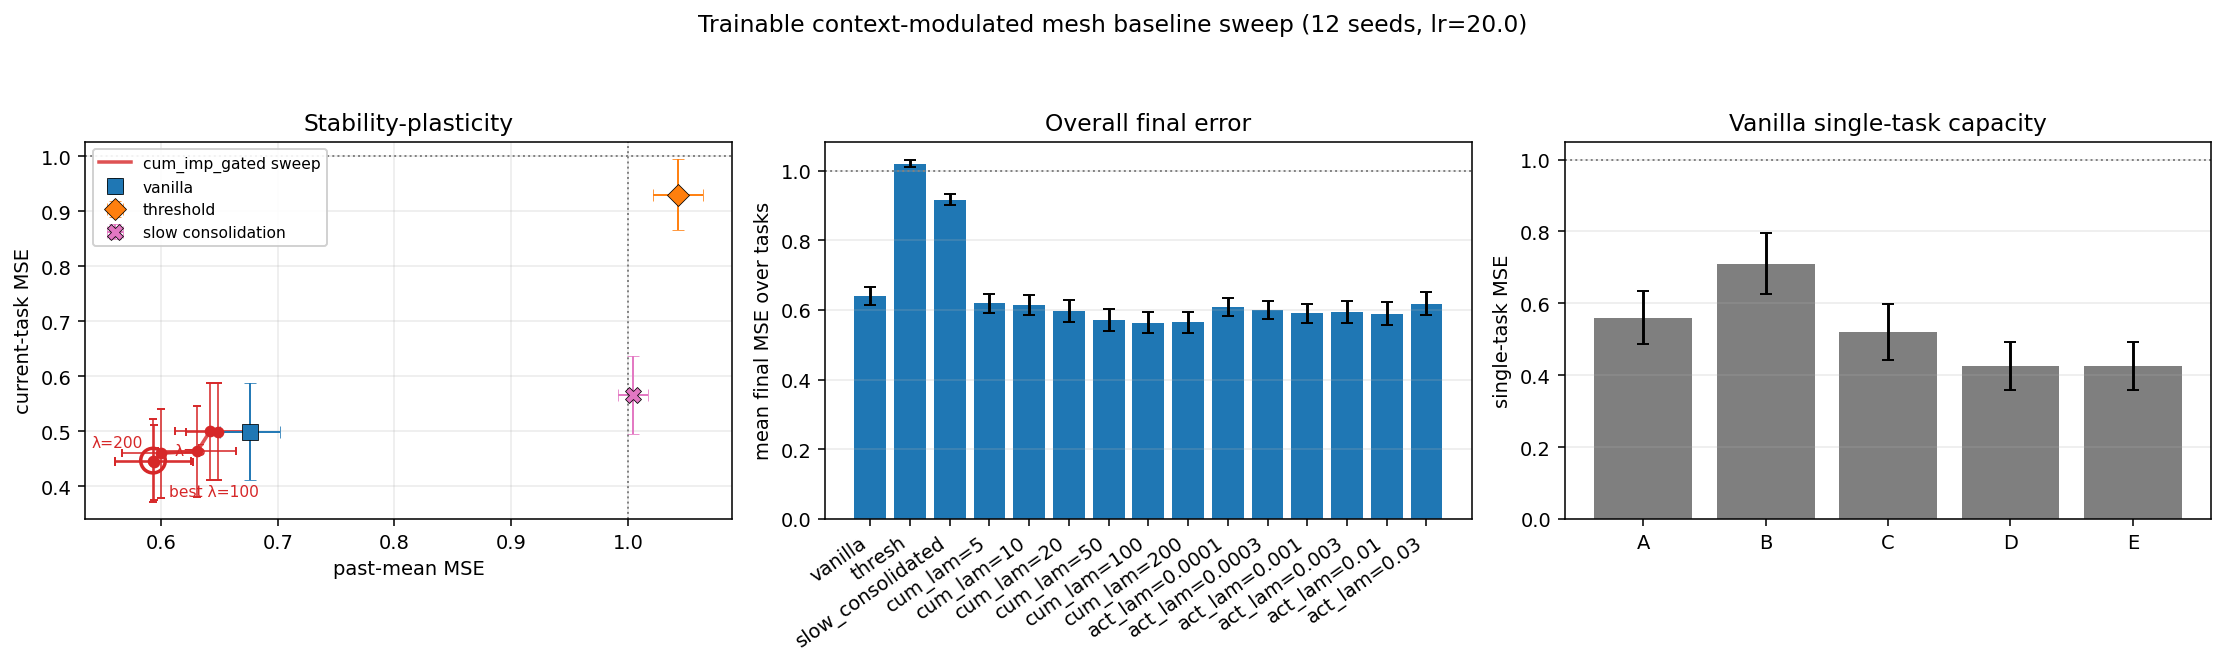
\includegraphics[width=\textwidth]{results/context_modulated_baseline_sweep.png}
\caption{Baseline sweep on the trainable context-modulated mesh. Left:
past-mean vs current-task MSE after the five-task sequence; the
cumulative-importance sweep traces a path that sits on the
Pareto-improving side of vanilla rather than along a
stability--plasticity trade. Middle: overall final MSE across rules.
Right: single-task vanilla capacity. Thresholding and slow
consolidation do not improve this benchmark.}
\label{fig:context-baseline}
\end{figure}

The main sequential results are:
\[
\begin{array}{lccc}
\toprule
\text{rule} & \text{past MSE} & \text{current MSE} & \text{overall MSE}\\
\midrule
\text{vanilla} & 0.676 & 0.499 & 0.641\\
\text{threshold} & 1.043 & 0.931 & 1.020\\
\text{slow consolidation} & 1.004 & 0.566 & 0.917\\
\text{cum. importance }(\lambda=5) & 0.649 & 0.499 & 0.619\\
\text{cum. importance }(\lambda=10) & 0.642 & 0.500 & 0.614\\
\text{cum. importance }(\lambda=20) & 0.631 & 0.463 & 0.597\\
\text{cum. importance }(\lambda=50) & 0.600 & 0.460 & 0.572\\
\text{cum. importance }(\lambda=100) & 0.593 & 0.447 & 0.564\\
\text{cum. importance }(\lambda=200) & 0.594 & 0.443 & 0.564\\
\bottomrule
\end{array}
\]

The best cumulative importance setting reduces overall final MSE from
$0.641$ for vanilla to $0.564$ at $\lambda=100$. In paired differences
against vanilla, this corresponds to
\[
\Delta \text{past} = -0.083 \pm 0.023,\qquad
\Delta \text{current} = -0.052 \pm 0.042,\qquad
\Delta \text{overall} = -0.077 \pm 0.020.
\]
Both past-task retention and current-task fit improve at the same
operating point, so cumulative local importance sits on the
Pareto-improving side rather than on a stability--plasticity tradeoff
frontier. Relative to the vanilla-to-single-task forgetting budget of
$0.641 - 0.529 \approx 0.112$, the best cumulative setting recovers
about $69\%$. The larger qualitative step was still correcting the
task formulation by making task context identifiable and trainable.

\section{Interpretation}

The current state of the project is best summarized as follows.

\begin{enumerate}
\item A passive edge-coupled mesh can be trained by purely local
contrastive gradients.
\item Continual learning benchmarks on this substrate require task
identifiability. Without context, five orthogonal regressions with the
same input distribution and same output pair are not a well-posed
memory problem.
\item A compact trainable context modulation mechanism makes the
five-task problem learnable without increasing the number of sensory
input nodes or adding separate output heads.
\item Scalar cumulative importance gives a Pareto improvement over
vanilla contrastive learning: at the chosen operating point both
past-task retention and current-task fit are better than vanilla,
recovering roughly $69\%$ of the vanilla-to-single-task forgetting
budget.
\item Simple thresholding and the current slow-consolidation rule do not
improve the contextual benchmark.
\end{enumerate}

This is a useful baseline, but not yet a final local learning rule.
Scalar squared-gradient importance is a Fisher-diagonal proxy: it
captures how strongly the loss curvature responds at each edge, but
not which edges the substrate is actually using to express a stored
task. Replacing it with importance signals built from local activity
signatures (free- and clamped-phase endpoint voltages, per-edge energy
contributions) is the natural next mechanism step.

\section{Next Steps}

\paragraph{Use local activity signatures.}
The next promising direction is to build importance from local activity
signatures rather than scalar gradient magnitudes alone. Each edge can
observe voltage drops in the free and clamped phases, the local
contrastive gradient, and the local context-modulated conductance. These
quantities define an edge-local signature of how that edge participates
in a task. A better rule should protect changes that would disrupt a
stored task signature while leaving compatible changes plastic.

\paragraph{Tune and compare against stronger baselines.}
The cumulative importance sweep should be repeated for longer sequences,
different context dimensions, and varied task overlap. The most useful
comparison is not whether a rule beats a zero-output baseline, but
whether it improves the stability-plasticity frontier over tuned vanilla
and tuned cumulative importance.

\paragraph{Biological plausibility.}
The trainable context sensitivity can be interpreted as a local
neuromodulatory gain: context changes how strongly each edge participates
in the network, while plasticity remains edge-local. Future rules should
move toward synaptic-tagging and metaplastic mechanisms: eligibility
traces, slow consolidation, and local activity-dependent protection,
rather than exact software-style Fisher penalties.

\begin{thebibliography}{99}

\bibitem{mccloskey1989}
M.\ McCloskey and N.\ J.\ Cohen.
\newblock Catastrophic interference in connectionist networks: The sequential
learning problem.
\newblock \emph{Psychology of Learning and Motivation}, 24:109--165, 1989.

\bibitem{kirkpatrick2017}
J.\ Kirkpatrick et al.
\newblock Overcoming catastrophic forgetting in neural networks.
\newblock \emph{Proceedings of the National Academy of Sciences},
114(13):3521--3526, 2017.

\bibitem{zenke2017}
F.\ Zenke, B.\ Poole, and S.\ Ganguli.
\newblock Continual learning through synaptic intelligence.
\newblock \emph{ICML}, 2017.

\bibitem{stern2022}
M.\ Stern, D.\ Hexner, J.\ W.\ Rocks, and A.\ J.\ Liu.
\newblock Supervised learning through physical changes in a mechanical system.
\newblock \emph{Physical Review X}, 12:031044, 2022.

\bibitem{stern2024}
M.\ Stern, A.\ J.\ Liu, and V.\ Balasubramanian.
\newblock Physical learning beyond the quasistatic limit.
\newblock \emph{Physical Review Research}, 6:013004, 2024.

\bibitem{scellier2017}
B.\ Scellier and Y.\ Bengio.
\newblock Equilibrium propagation: Bridging the gap between energy-based
models and backpropagation.
\newblock \emph{Frontiers in Computational Neuroscience}, 11:24, 2017.

\bibitem{thresholdedphysical2025}
Authors.
\newblock Thresholded local updates in tunable physical networks for
sequential learning.
\newblock \emph{arXiv:2512.03799}, 2025.

\end{thebibliography}

\end{document}
